The given polynomial can be expressed as the parabola 
\begin{align}
\vec{x}^T 
\myvec{
1 & 0 \\
0 & 0
}
\vec{x} + 
\myvec{
-2 & 0 
}
\vec{x} + 0 = 0 \label{eq:5.1.2_conics_main}
\end{align}


\begin{align}
\because \myvec{0&0}
\myvec{
1 & 0 \\
0 & 0
}
\myvec{0\\0} &+ 
\myvec{
-2 & 0 
}
\myvec{0\\0}   = 0
\end{align}
0 is a root.
\begin{align}
\because \myvec{2&0}
\myvec{
1 & 0 \\
0 & 0
}
\myvec{2\\0} &+ 
\myvec{
-2 & 0 
}
\myvec{2\\0}  =  0
\end{align}
2 is also a root.  This is verified by plotting Fig. \ref{fig:5.1.2_quadeq_conics_example}
through the following code.
\begin{lstlisting}
solutions/2/codes/conics_example/conics.py
\end{lstlisting}

 \begin{figure}[!ht]
\centering
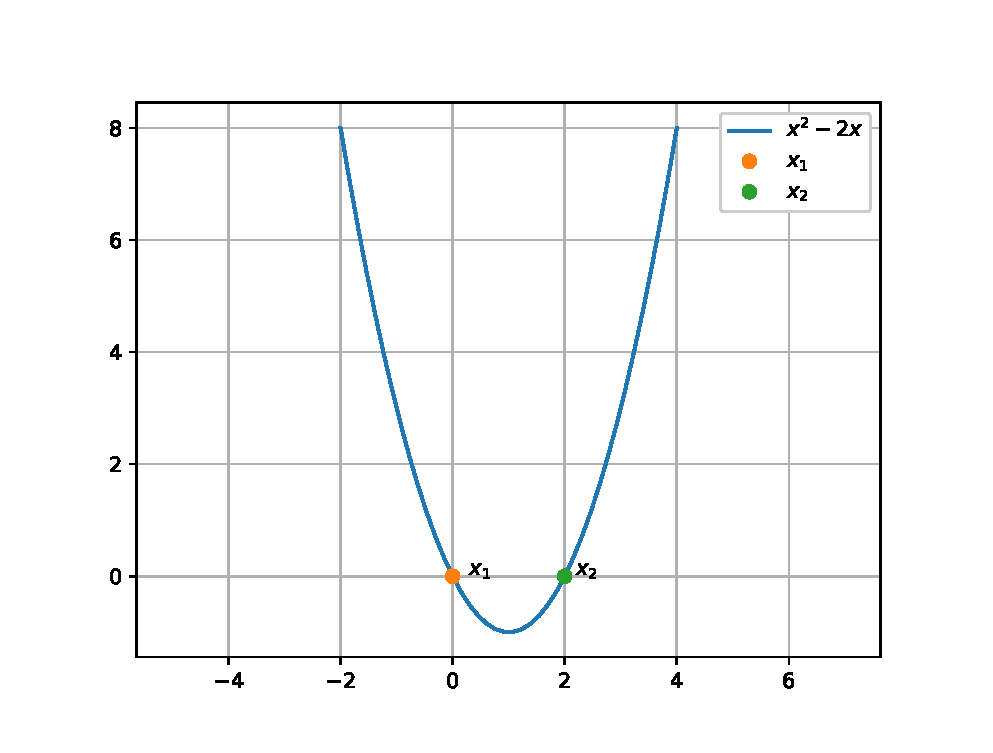
\includegraphics[width=\columnwidth]{./solutions/2/figs/conics_example/quadratic_equation.eps}
\caption{}
\label{fig:5.1.2_quadeq_conics_example}
\end{figure} 
